\documentclass{../../slides-style}

\slidetitle{Лекция 4: Работа с требованиями}{12.03.2024}

\begin{document}

    \begin{frame}[plain]
        \titlepage
    \end{frame}

    \begin{frame}
        \frametitle{Требования}
        Требование --- это любое условие, которому должна соответствовать разрабатываемая система или программное средство
        \begin{itemize}
            \item Возможности
            \item Ограничения
        \end{itemize}
    \end{frame}

    \begin{frame}
        \frametitle{Виды требований}
        \begin{center}
            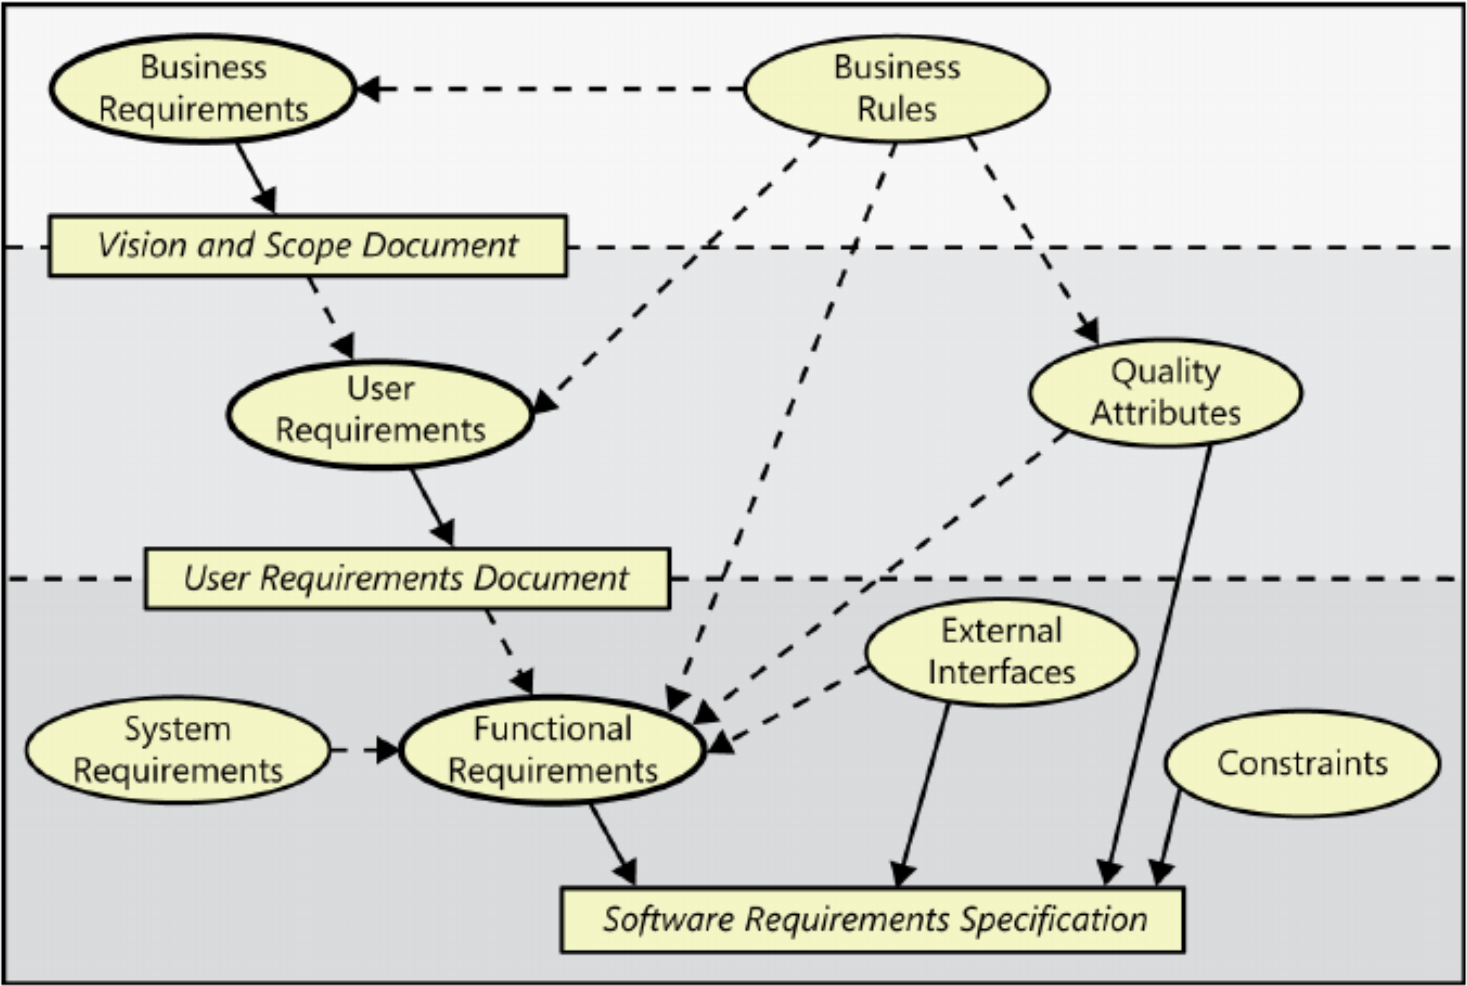
\includegraphics[width=0.8\textwidth]{requirements.png}
        \end{center}
    \end{frame}

    \begin{frame}
        \frametitle{Пример}
        \begin{itemize}
            \item Бизнес-требование:
            \begin{itemize}
                \item продукт позволит пользователям эффективно исправлять орфографические ошибки в тексте
            \end{itemize}
            \item Требования пользователей:
            \begin{itemize}
                \item сценарии ``Найти орфографическую ошибку'' или ``Добавить слово в общий словарь''
            \end{itemize}
            \item Функциональные требования:
            \begin{itemize}
                \item поиск и выделение слова с ошибкой
                \item отображение диалогового окна с фрагментом текста с ошибочным словом
                \item полнотекстовая замена слова с ошибкой
            \end{itemize}
            \item Атрибуты качества:
            \begin{itemize}
                \item простота использования (``эффективность'')
            \end{itemize}
        \end{itemize}
    \end{frame}

    \begin{frame}
        \frametitle{Основные риски, связанные с требованиями}
        \begin{itemize}
            \item Недостаточное вовлечение пользователей
            \item Игнорирование классов пользователей
            \item Разрастание требований пользователей
            \item Двусмысленность требований
            \item Излишняя дополнительная функциональность
            \item Урезанная спецификация
            \item Небрежное планирование
        \end{itemize}
    \end{frame}

    \begin{frame}
        \frametitle{Требования к требованиям}
        \begin{itemize}
            \item Единичность
            \item Завершенность
            \item Непротиворечивость
            \item Атомарность
            \item Отслеживаемость
            \item Актуальность
            \item Выполнимость
            \item Недвусмысленность
            \item Обязательность
            \item Проверяемость
        \end{itemize}
    \end{frame}

    \begin{frame}
        \frametitle{Работа с требованиями}
        \begin{columns}
            \begin{column}{0.4\textwidth}
                \begin{itemize}
                    \item разработка требований
                    \begin{itemize}
                        \item выявление требований
                        \item анализ требований
                        \item спецификация требований
                        \item проверка требований
                    \end{itemize}
                    \item управление требованиями
                \end{itemize}
            \end{column}
            \begin{column}{0.6\textwidth}
                \strut
                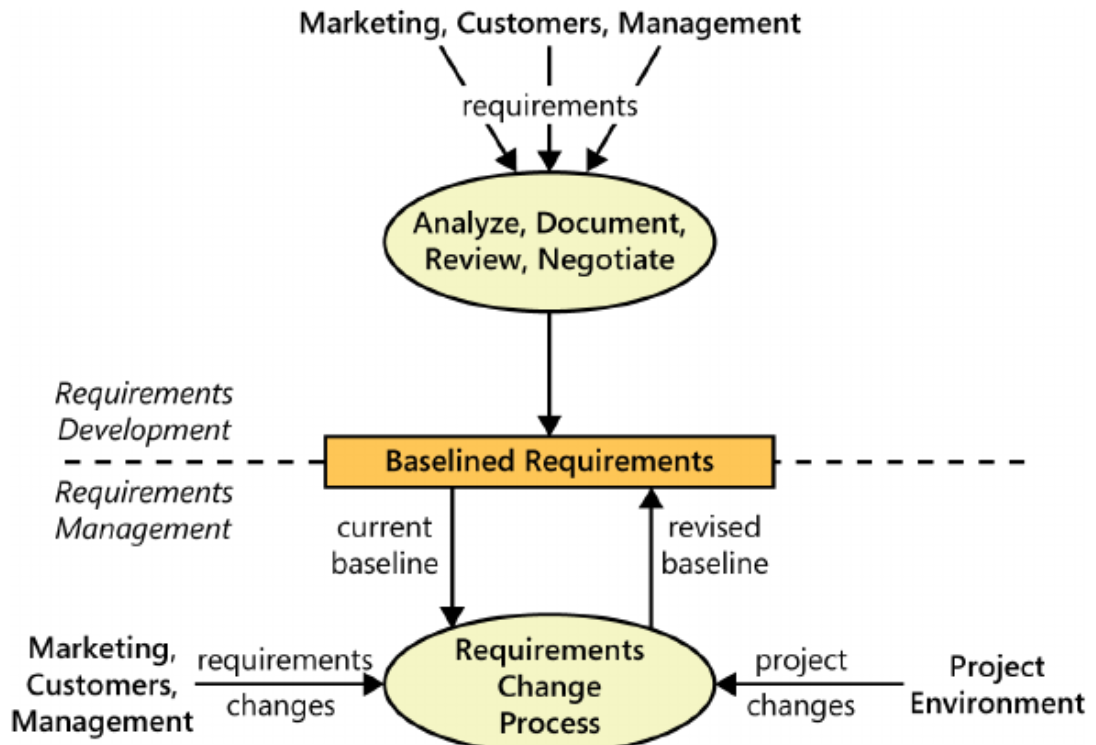
\includegraphics[width=\textwidth]{requirementsProcess.png}
            \end{column}
        \end{columns}
    \end{frame}

    \begin{frame}
        \frametitle{Выявление требований}
        \begin{itemize}
            \item Определение процесса формулирования требований
            \item Определение классов пользователей и их характеристик
            \item Выбор типичного пользователя в каждом классе пользователей
            \item Организация фокус-групп/интервью типичных пользователей
            \item Наблюдение за пользователями на рабочих местах
            \item Изучение отчетов о проблемах работающих систем
            \item Определение системных событий и реакции на них
            \item Создание документа об образе и границах проекта
        \end{itemize}
    \end{frame}

    \begin{frame}
        \frametitle{Выявление требований в реальности}
        \begin{center}
            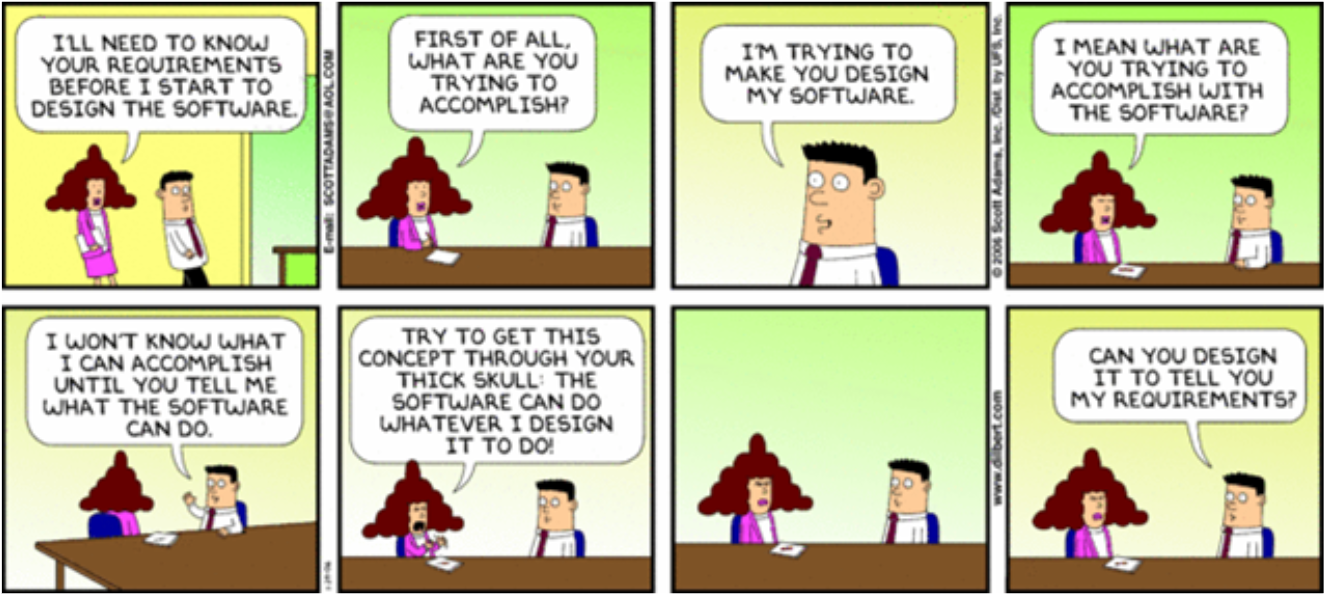
\includegraphics[width=0.8\textwidth]{aliceAndRequirements.png}
        \end{center}
    \end{frame}

    \begin{frame}
        \frametitle{Анализ требований}
        \begin{itemize}
            \item Анализ осуществимости требований
            \item Определение приоритетов требований
            \item Моделирование требований
            \item Создание словаря терминов
            \item Создание контекстной диаграммы
            \item Создание пользовательского интерфейса и технических прототипов
        \end{itemize}
    \end{frame}

    \begin{frame}
        \frametitle{Проверка требований}
        \begin{itemize}
            \item Изучение документов с требованиями
            \item Определение критериев приемлемости
            \item Тестирование требований
        \end{itemize}
    \end{frame}

    \begin{frame}
        \frametitle{Процесс работы с требованиями}
        \begin{center}
            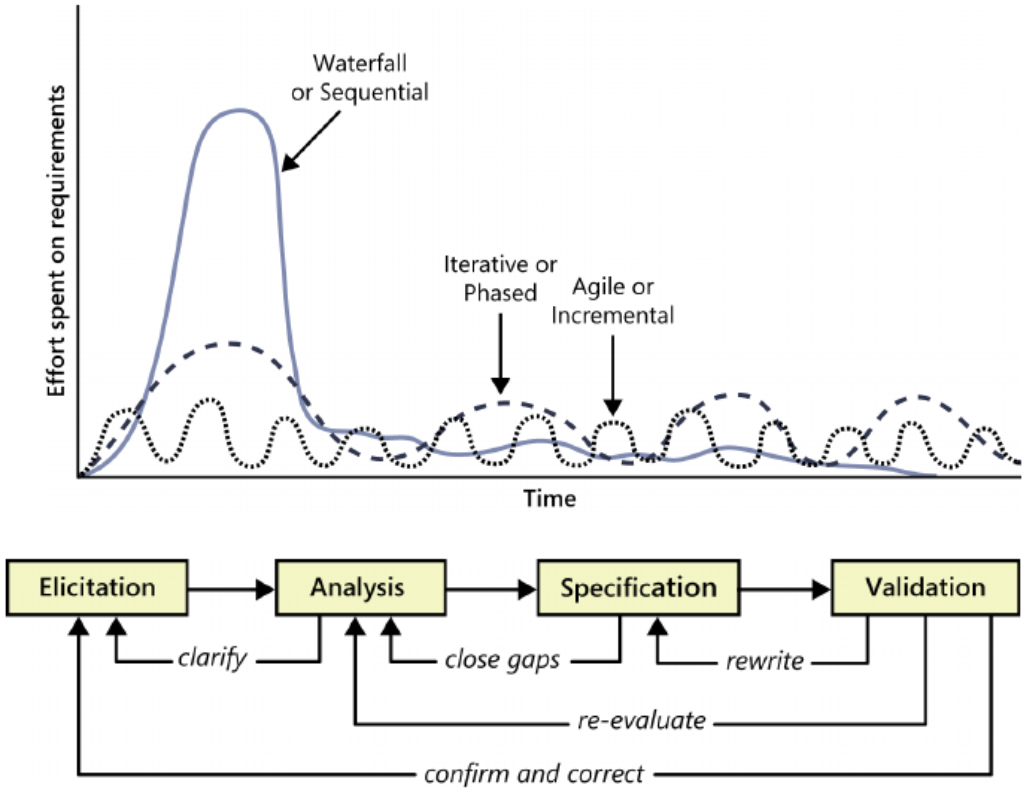
\includegraphics[width=0.8\textwidth]{requirementsProcess2.png}
        \end{center}
    \end{frame}

    \begin{frame}
        \frametitle{Навыки, необходимые аналитику}
        \begin{itemize}
            \item Умение задавать вопросы
            \item Умение слушать
            \item Умение наблюдать
            \item Навыки межличностного общения
            \item Навыки анализа
            \item Навыки написания документации
            \item Навыки моделирования
            \item Организационные навыки
            \item Творческий подход
        \end{itemize}
    \end{frame}

    \begin{frame}
        \frametitle{Трудовые функции аналитика}
        \framesubtitle{Профстандарт 06.022 <<Системный аналитик>>}
        \begin{itemize}
            \item Разработка и сопровождение требований к отдельным функциям системы
            \item Разработка и сопровождение требований и технических заданий на разработку и модернизацию систем и подсистем малого и среднего масштаба и сложности
            \item Концептуальное, функциональное и логическое проектирование систем среднего и крупного масштаба и сложности
            \item Управление аналитическими работами и подразделением
        \end{itemize}
        Квалификационные уровни с 4 по 7
    \end{frame}

    \begin{frame}
        \frametitle{Создаваемые документы}
        \begin{itemize}
            \item Документ об образе и границах системы
            \item Глоссарий
            \item Модель требований
            \item Прототип пользовательского интерфейса
            \item Спецификация требований
        \end{itemize}
    \end{frame}

    \begin{frame}
        \frametitle{Документ об образе и границах проекта}
        \begin{columns}
            \begin{column}{0.5\textwidth}
                \begin{itemize}
                    \item Бизнес-требования
                    \begin{itemize}
                        \item Контекст
                        \item Бизнес-возможности
                        \item Бизнес-цели и критерии успеха
                        \item Потребности клиента или рынка
                        \item Бизнес-риски
                    \end{itemize}
                    \item Project vision
                    \begin{itemize}
                        \item Положение об образе проекта
                        \item Основные функции
                        \item Предположения и зависимости
                    \end{itemize}
                \end{itemize}
            \end{column}
            \begin{column}{0.5\textwidth}
                \begin{itemize}
                    \item Масштабы и ограничения проекта
                    \begin{itemize}
                        \item Основная функциональность
                        \item Объем первоначальной версии
                        \item Объем последующих версий
                        \item Ограничения и исключения
                    \end{itemize}
                    \item Бизнес-контекст
                    \begin{itemize}
                        \item Профили заинтересованных лиц
                        \item Приоритеты проекта
                        \item Операционная среда
                    \end{itemize}
                \end{itemize}
            \end{column}
        \end{columns}
    \end{frame}

    \begin{frame}
        \frametitle{Контекстная диаграмма}
        \begin{columns}
            \begin{column}{0.4\textwidth}
                Задание границ системы и связи с внешним миром
            \end{column}
            \begin{column}{0.6\textwidth}
                \strut
                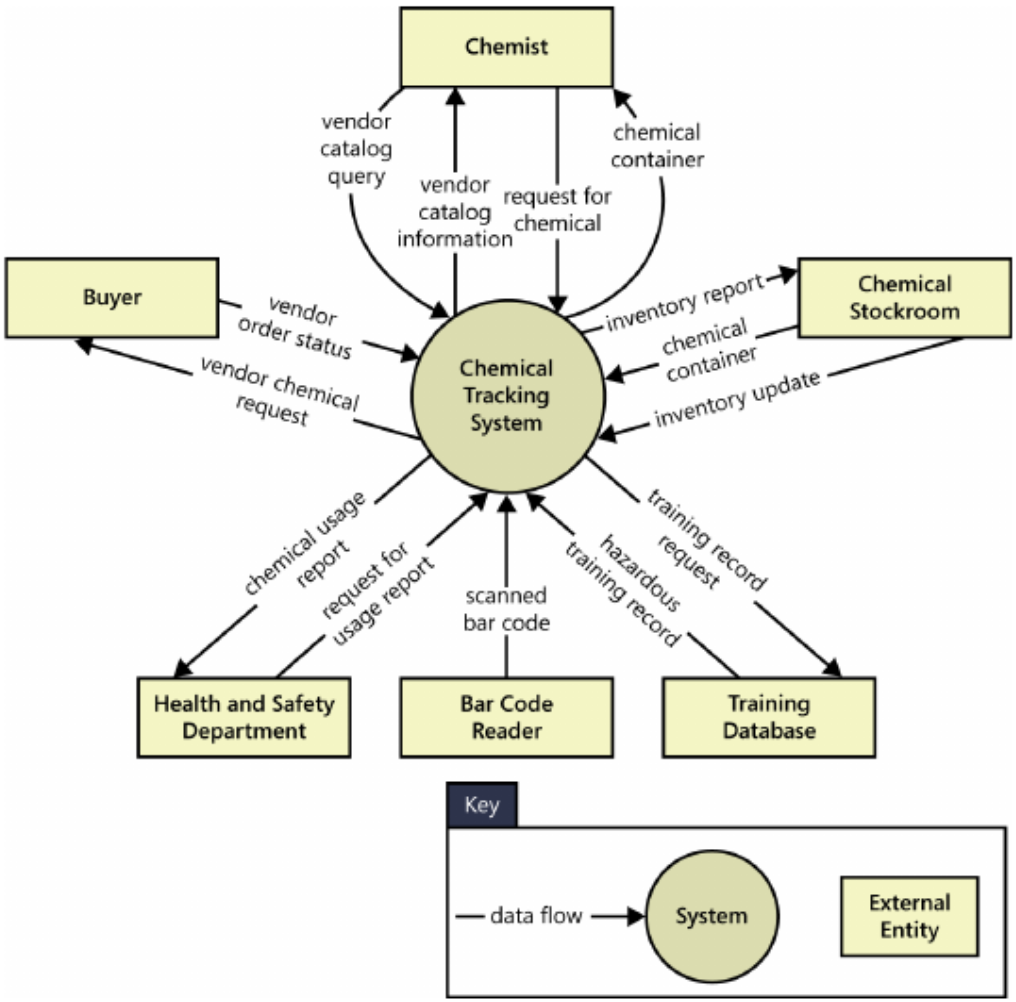
\includegraphics[width=\textwidth]{contextDiagram.png}
            \end{column}
        \end{columns}
    \end{frame}

    \begin{frame}
        \frametitle{Feature tree}
        \begin{center}
            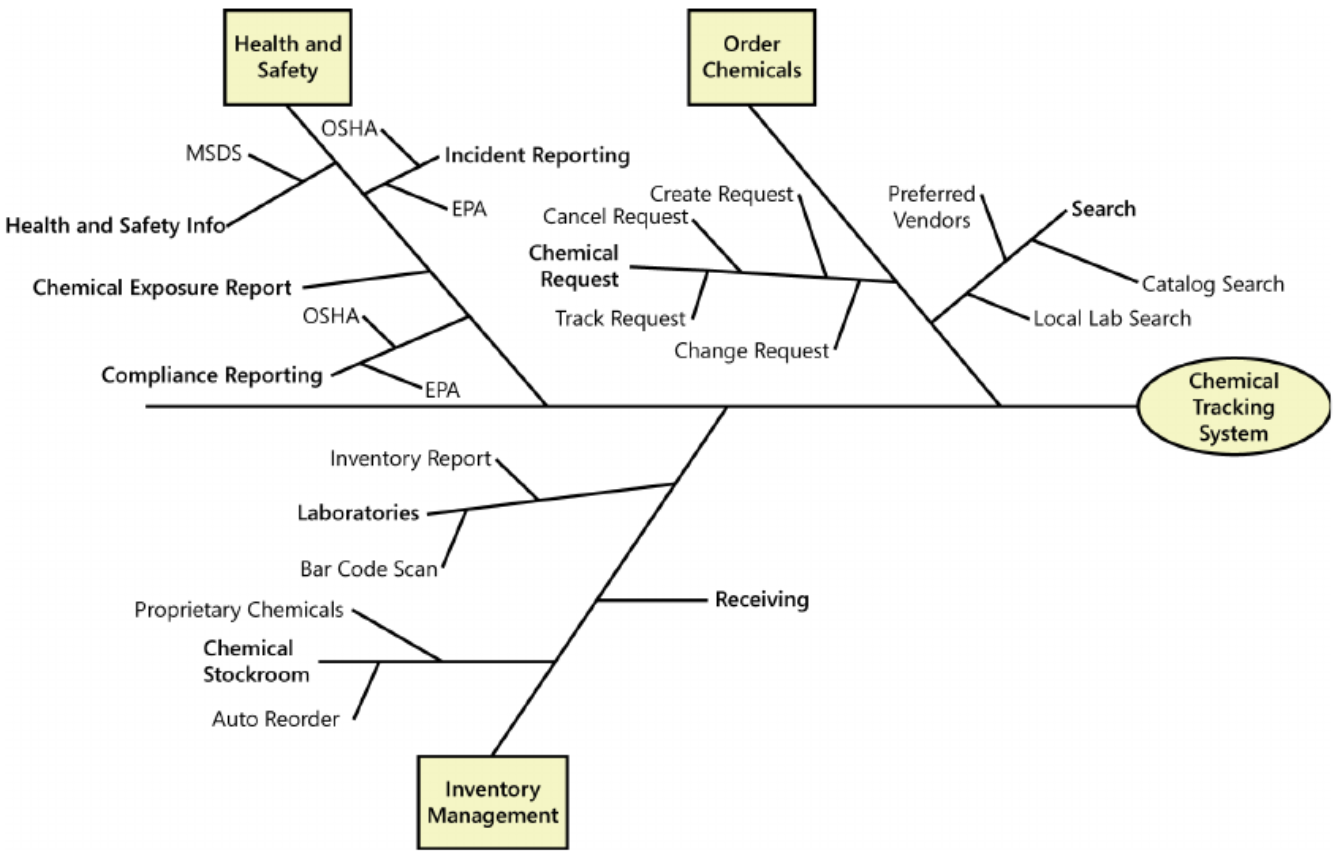
\includegraphics[width=0.8\textwidth]{featureTree.png}
        \end{center}
    \end{frame}

    \begin{frame}
        \frametitle{Моделирование требований}
        \begin{itemize}
            \item Диаграммы случаев использования
            \begin{itemize}
                \item Актёры (роли)
                \begin{itemize}
                    \item кто-то или что-то вне системы, влияющий или оказывающий влияние
                    \item люди или программные системы
                \end{itemize}
                \item Случаи (сценарии) использования
                \begin{itemize}
                    \item цель пользователя системы
                    \item действие-реакция для достижения цели
                \end{itemize}
            \end{itemize}
            \item Общее представление функциональных требований
        \end{itemize}
        \begin{center}
            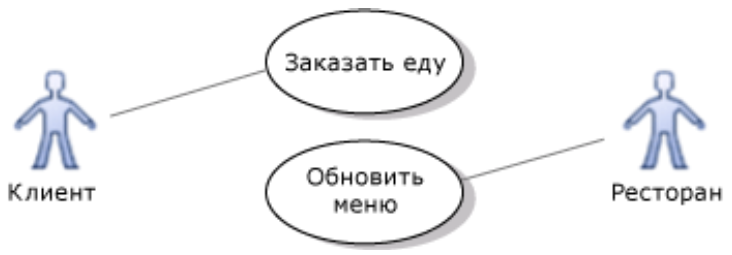
\includegraphics[width=0.6\textwidth]{useCaseSmallExample.png}
        \end{center}
    \end{frame}

    \begin{frame}
        \frametitle{Задание границ проекта}
        \begin{center}
            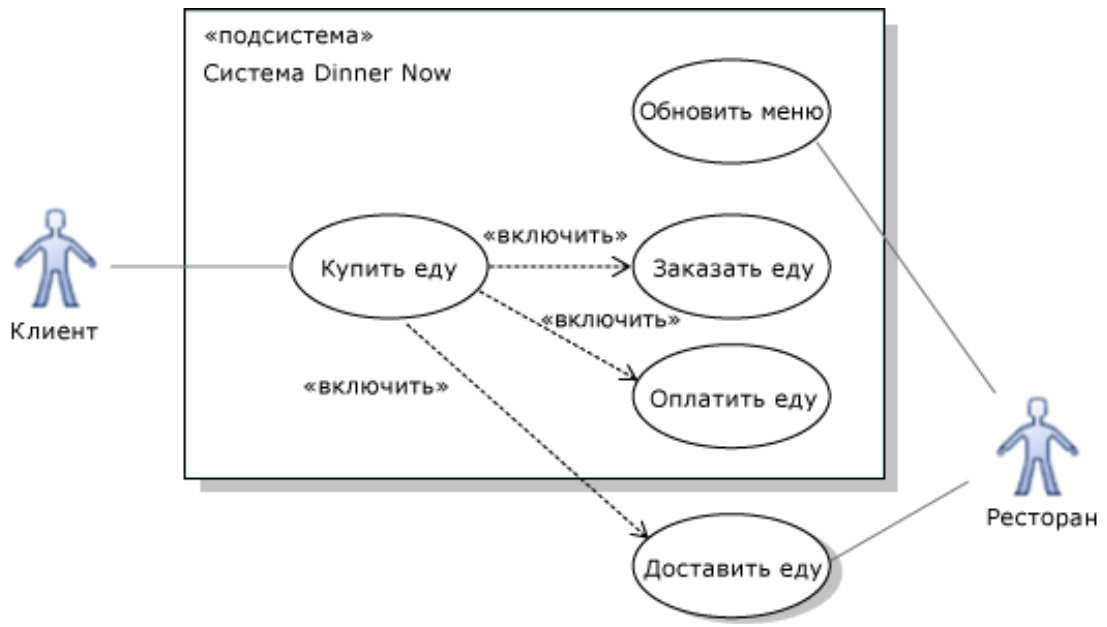
\includegraphics[width=0.9\textwidth]{useCaseBiggerExample.png}
        \end{center}
    \end{frame}

    \begin{frame}
        \frametitle{Сценарий использования (1)}
        \begin{center}
            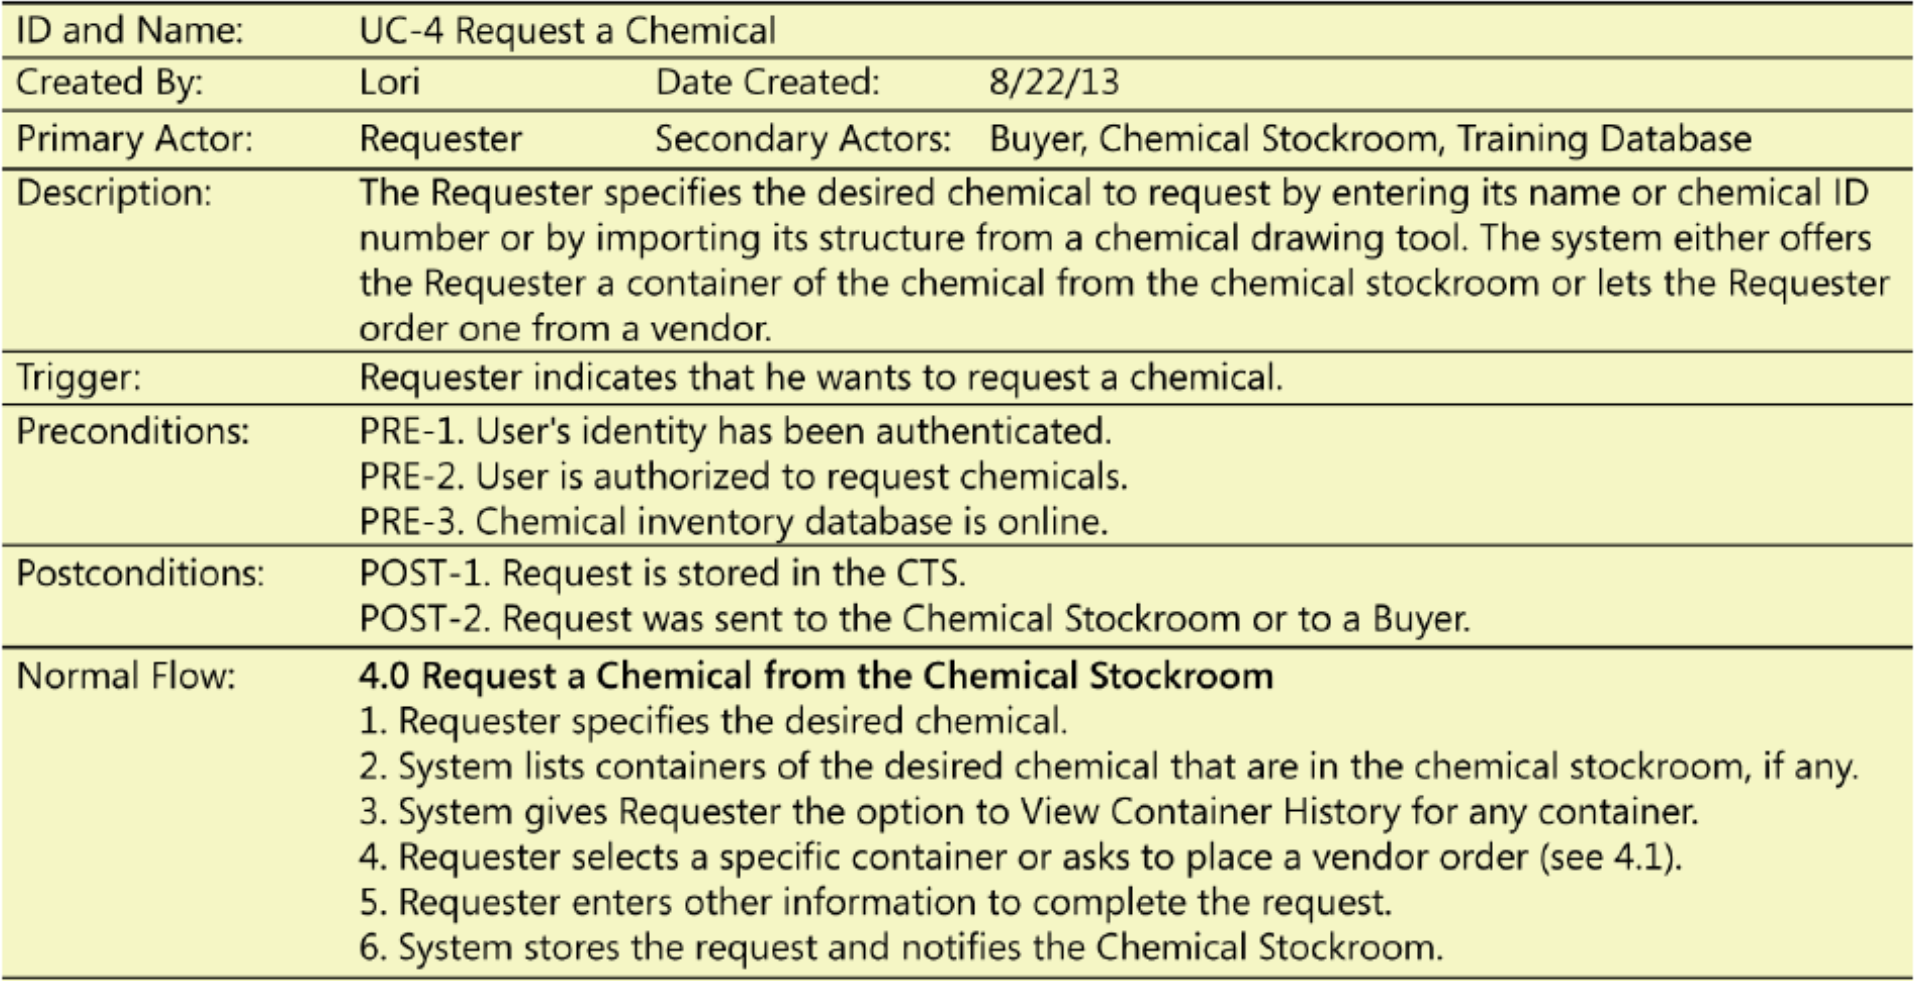
\includegraphics[width=\textwidth]{userScenario1.png}
        \end{center}
    \end{frame}

    \begin{frame}
        \frametitle{Сценарий использования (2)}
        \begin{center}
            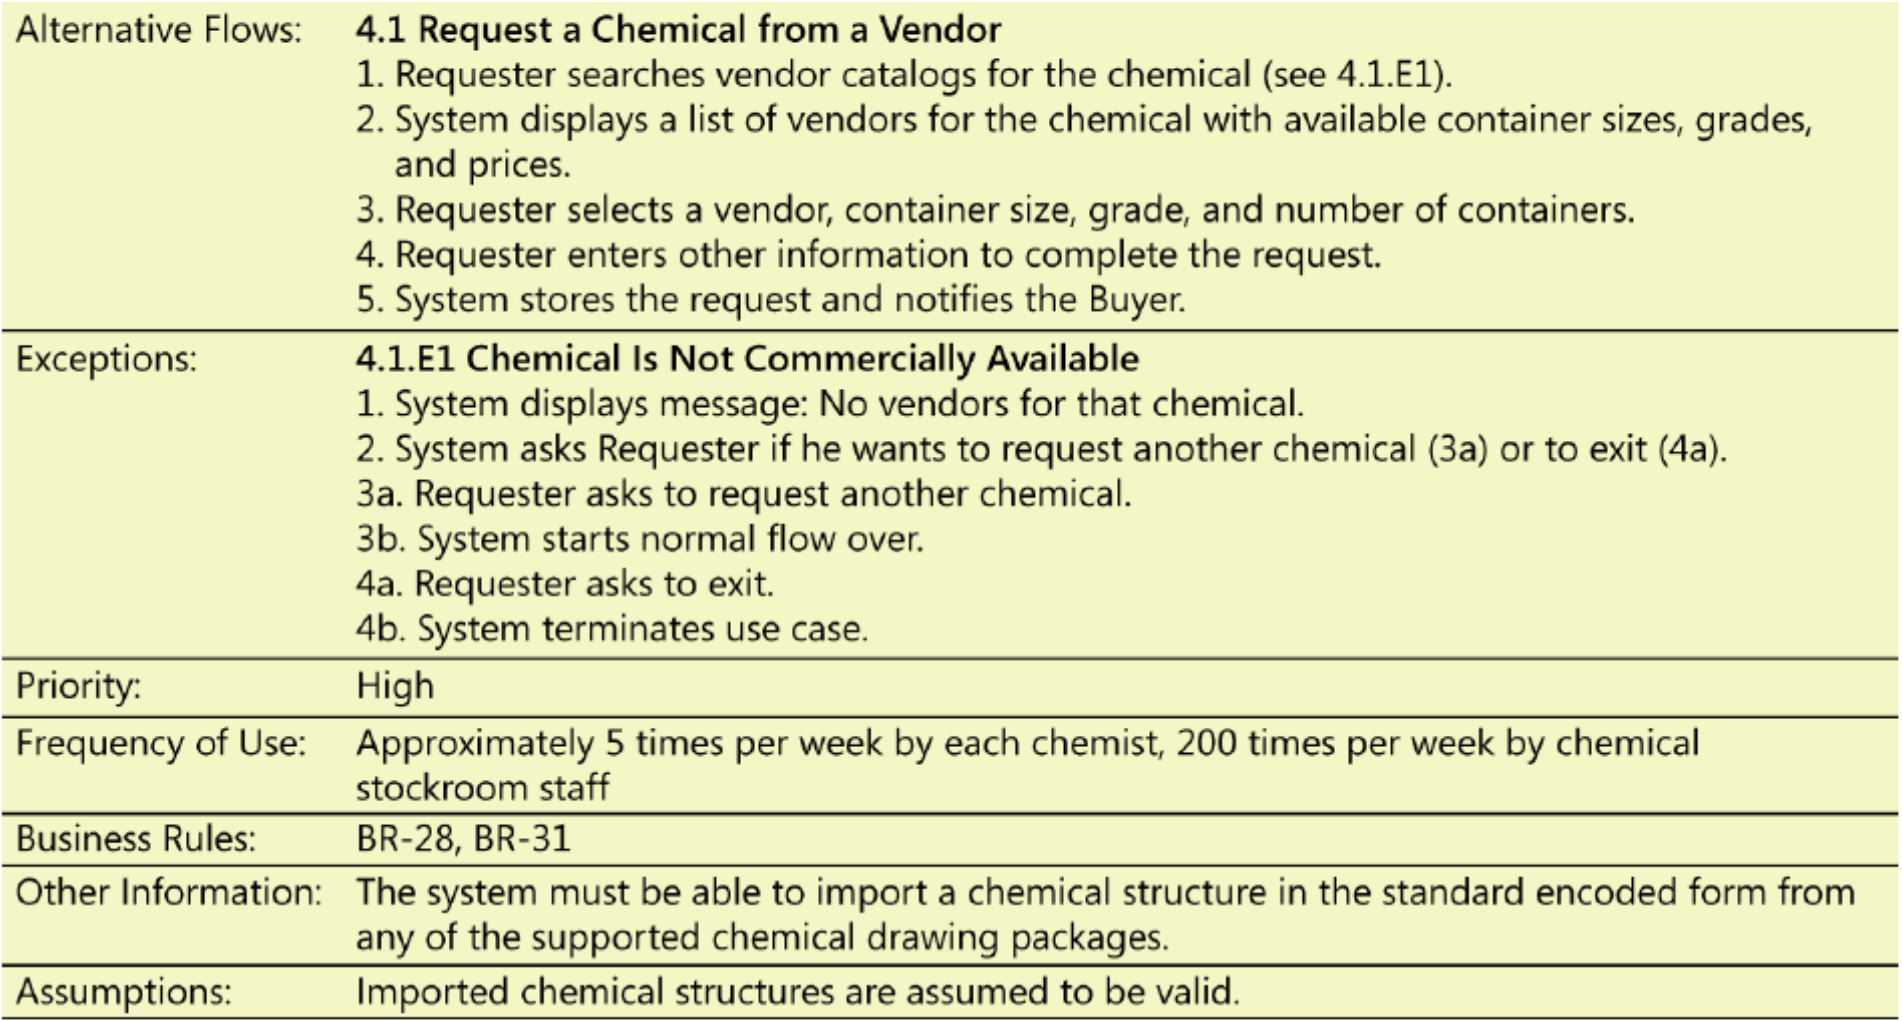
\includegraphics[width=\textwidth]{userScenario2.png}
        \end{center}
    \end{frame}

    \begin{frame}
        \frametitle{Диаграммы активности}
        \begin{center}
            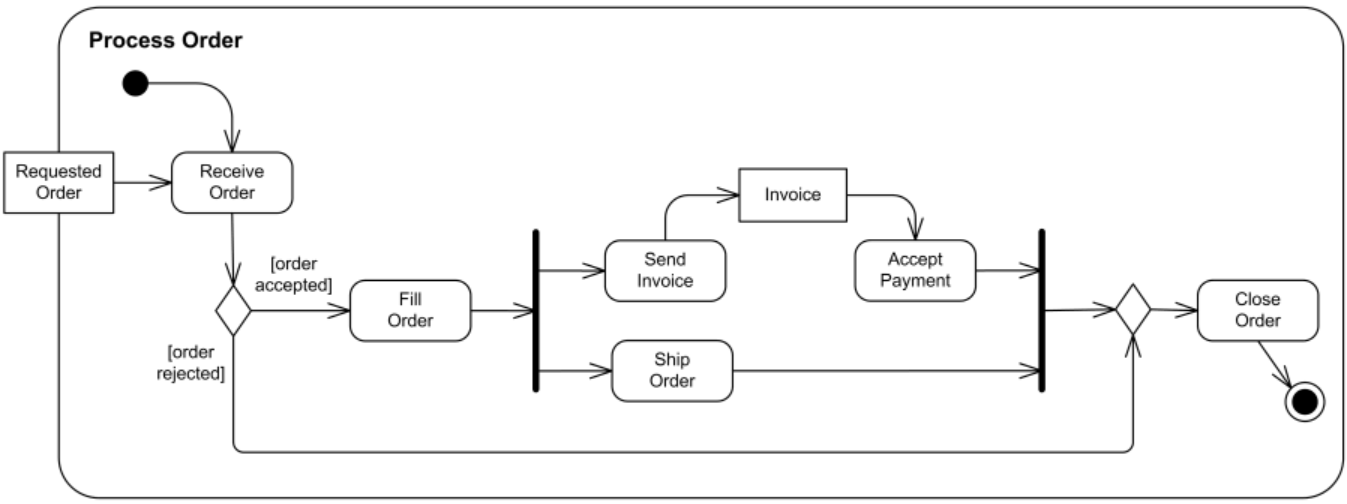
\includegraphics[width=\textwidth]{activity.png}
            \attribution{\url{https://www.uml-diagrams.org/}}
        \end{center}
    \end{frame}

    \begin{frame}
        \frametitle{Data-flow diagrams}
        \begin{columns}
            \begin{column}{0.4\textwidth}
                \begin{itemize}
                    \item сущности системы
                    \item внешние сущности
                    \item потоки данных
                    \item иерархическая модель
                \end{itemize}
            \end{column}
            \begin{column}{0.6\textwidth}
                \strut
                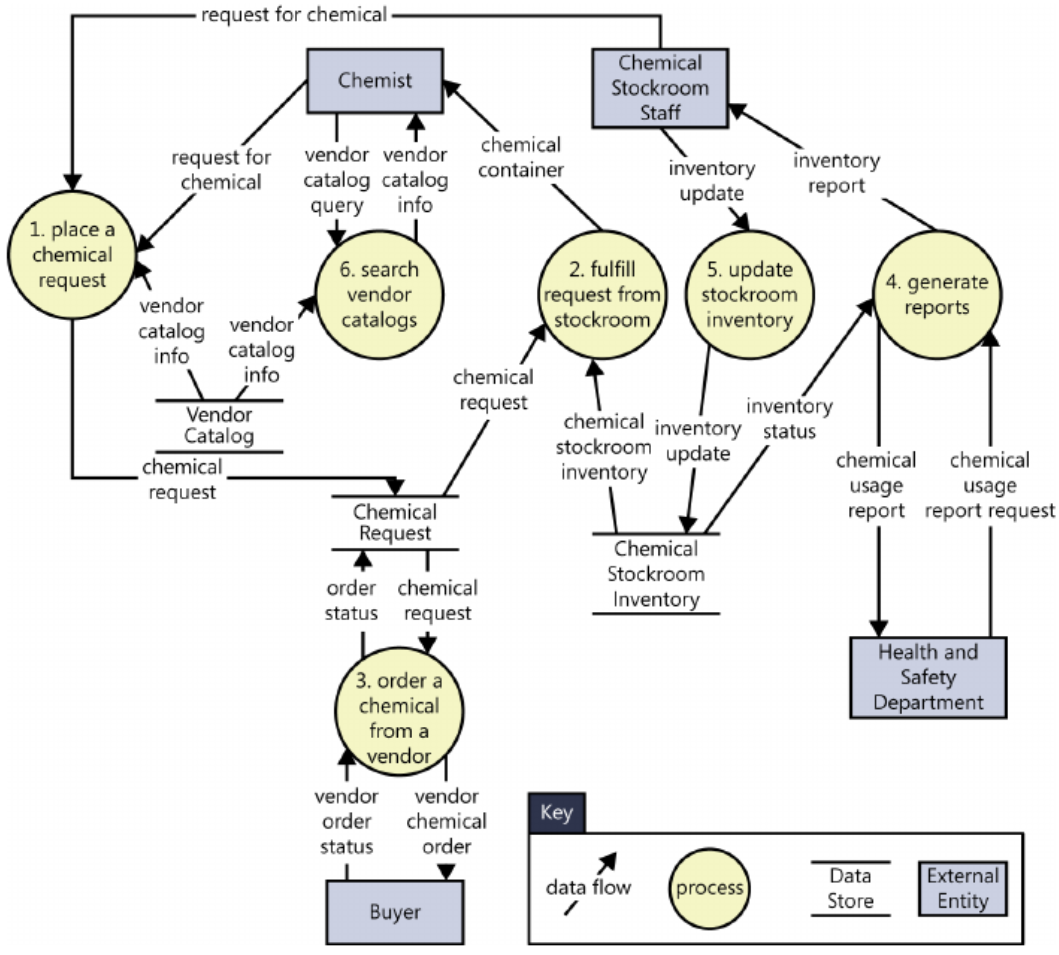
\includegraphics[width=\textwidth]{dfd.png}
            \end{column}
        \end{columns}
    \end{frame}

    \begin{frame}
        \frametitle{Диаграмма состояний}
        \begin{columns}
            \begin{column}{0.4\textwidth}
                \begin{itemize}
                    \item описание реактивных систем
                    \begin{itemize}
                        \item состояния
                        \item внешние события
                        \item переходы
                    \end{itemize}
                \end{itemize}
            \end{column}
            \begin{column}{0.6\textwidth}
                \strut
                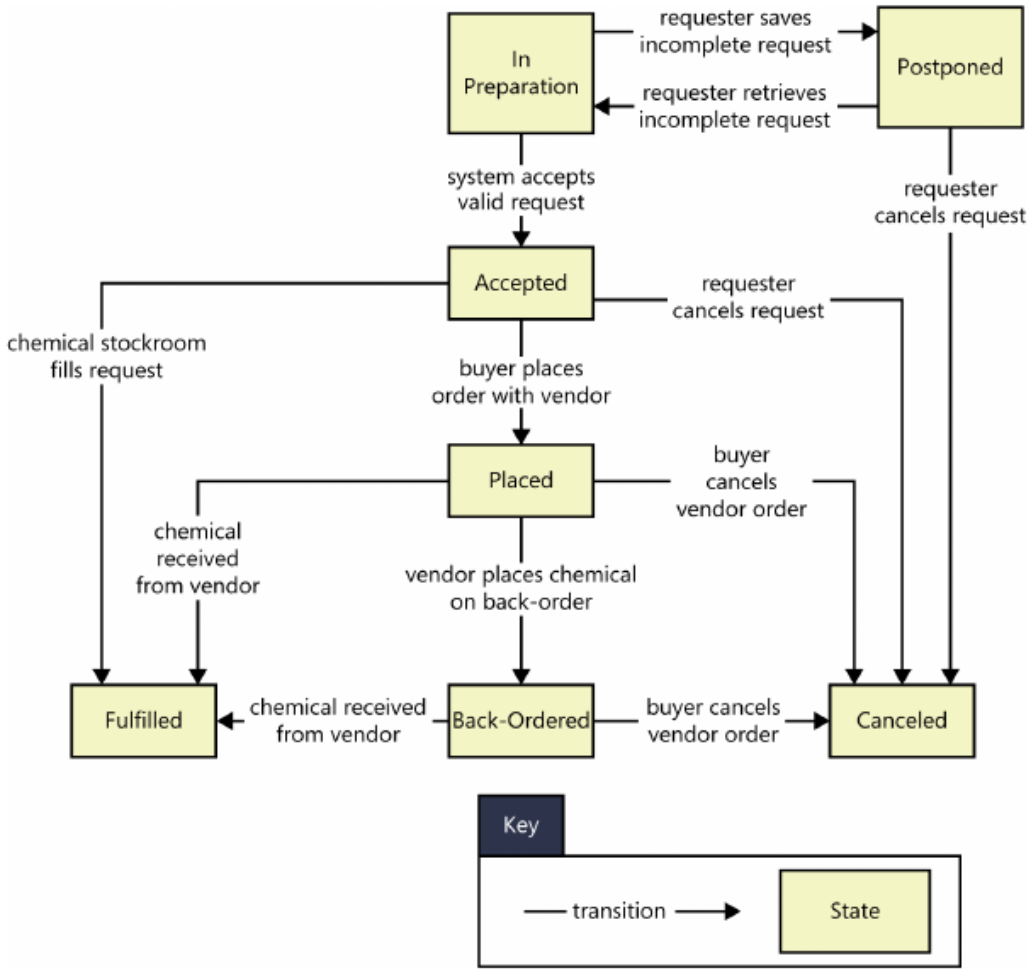
\includegraphics[width=\textwidth]{stateDiagram.png}
            \end{column}
        \end{columns}
    \end{frame}

    \begin{frame}
        \frametitle{Деревья решений}
        \begin{center}
            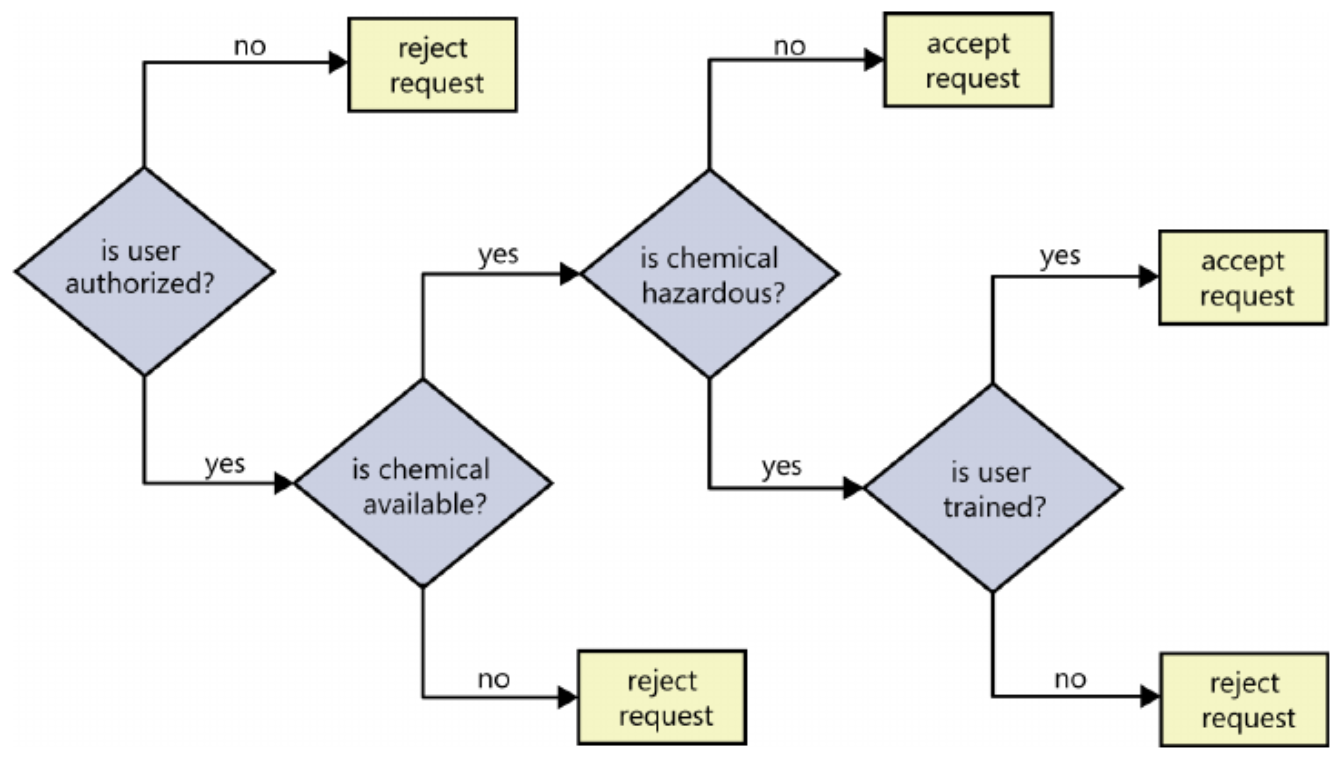
\includegraphics[width=0.8\textwidth]{decisionTrees.png}
        \end{center}
    \end{frame}

    \begin{frame}
        \frametitle{Спецификация требований к ПО (SRS) (1)}
        \begin{footnotesize}
            \begin{itemize}
                \item Введение
                \begin{itemize}
                    \begin{footnotesize}
                        \item Цели
                        \item Соглашения о терминах
                        \item Предполагаемая аудитория
                        \item Масштаб проекта
                        \item Ссылки на источники
                    \end{footnotesize}
                \end{itemize}
                \item Общее описание
                \begin{itemize}
                    \begin{footnotesize}
                        \item Видение продукта
                        \item Функциональность продукта
                        \item Классы и характеристики пользователей
                        \item Среда функционирования продукта
                        \item Рамки, ограничения, правила и стандарты
                        \item Документация для пользователей
                        \item Допущения и зависимости
                    \end{footnotesize}
                \end{itemize}
            \end{itemize}
        \end{footnotesize}
    \end{frame}

    \begin{frame}
        \frametitle{Спецификация требований к ПО (SRS) (2)}
        \begin{footnotesize}
            \begin{itemize}
                \item Функциональность системы
                \begin{itemize}
                    \begin{footnotesize}
                        \item Функциональный блок X
                        \item Описание и приоритет
                        \item Причинно-следственные связи, алгоритмы
                        \item Функциональные требования
                    \end{footnotesize}
                \end{itemize}
                \item Требования к внешним интерфейсам
                \begin{itemize}
                    \begin{footnotesize}
                        \item Интерфейсы пользователя (UX)
                        \item Программные интерфейсы
                        \item Интерфейсы оборудования
                        \item Интерфейсы связи и коммуникации
                    \end{footnotesize}
                \end{itemize}
                \item Нефункциональные требования
                \begin{itemize}
                    \begin{footnotesize}
                        \item Требования к производительности
                        \item Требования к сохранности (данных)
                        \item Критерии качества ПО
                        \item Требования к безопасности системы
                    \end{footnotesize}
                \end{itemize}
                \item Прочие требования
            \end{itemize}
        \end{footnotesize}
    \end{frame}

    \begin{frame}
        \frametitle{Требования и тестирование}
        \begin{center}
            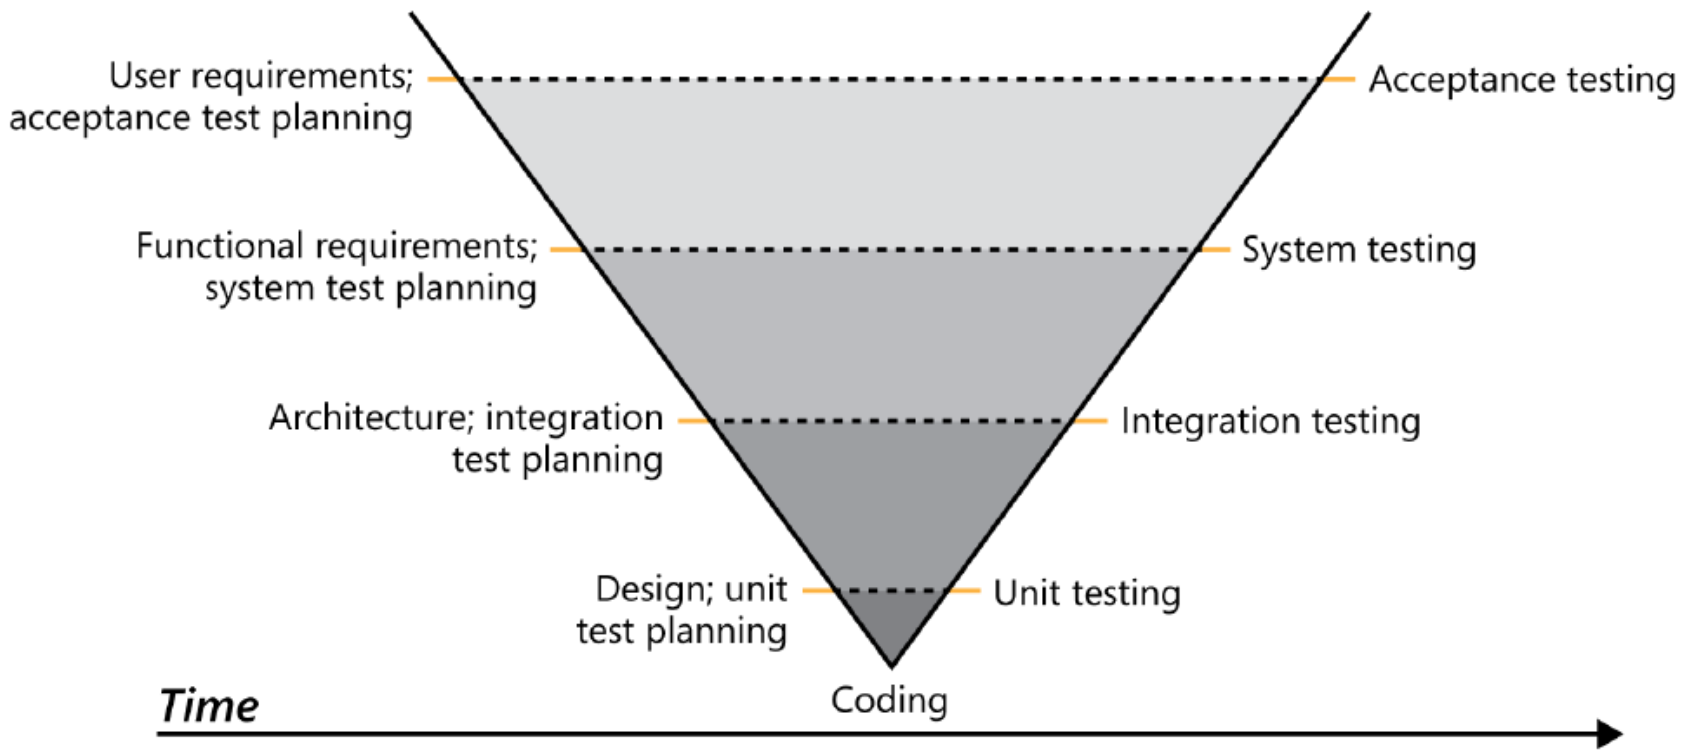
\includegraphics[width=\textwidth]{requirementsAndTesting.png}
        \end{center}
    \end{frame}

    \begin{frame}
        \frametitle{Управление требованиями}
        \begin{itemize}
            \item Определение процесса управления изменениями
            \item Создание базовой версии и управление версиями требований
            \item Использование средств версионирования и управления требованиями
            \item Анализ влияния изменений требований
            \item Оценка изменяемости требований
        \end{itemize}
        \begin{center}
            
\includegraphics[width=0.8\textwidth]{dilbertAndRequirementsManagement.png}
        \end{center}
    \end{frame}

    \begin{frame}
        \frametitle{Не соглашайтесь, будьте как Уолли}
        \begin{center}
            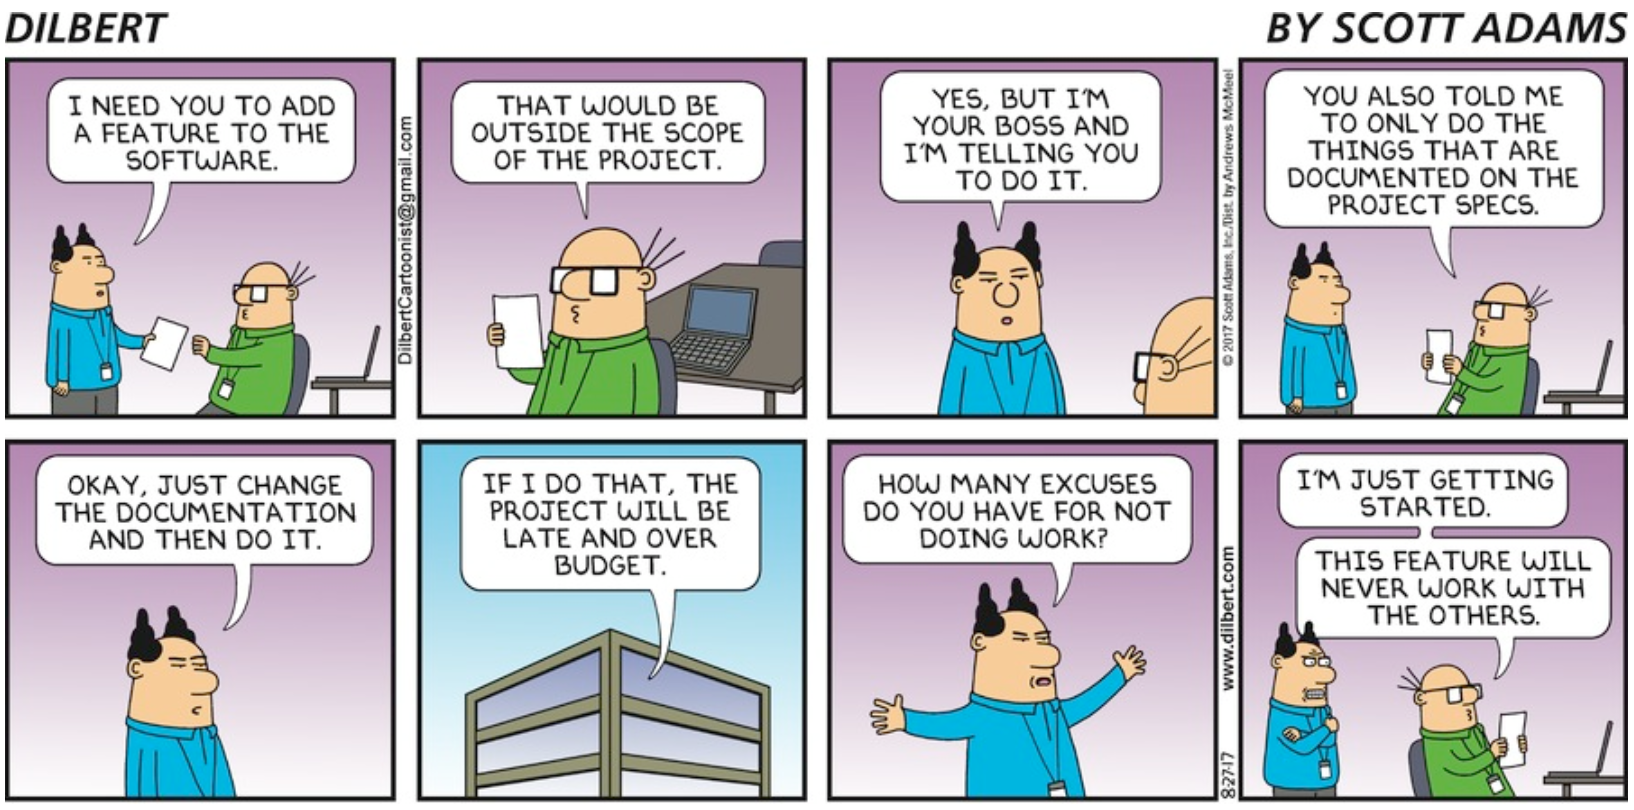
\includegraphics[width=0.8\textwidth]{requirementsAndWally.png}
        \end{center}
    \end{frame}

    \begin{frame}
        \frametitle{Атрибуты требований}
        \begin{itemize}
            \item Дата создания, автор
            \item Номер текущей ревизии
            \item Лицо, ответственное за удовлетворение требования
            \item Происхождение или источник требования
            \item Состояние (proposed, approved, implemented, verified, rejected и т.п.)
            \item Приоритет
            \item Подсистемы, для которых актуально требование
            \item Номер версии продукта, для которой актуально требование
            \item Критерий приемлемости, используемый метод проверки
        \end{itemize}
    \end{frame}

    \begin{frame}
        \frametitle{График сгорания}
        \begin{center}
            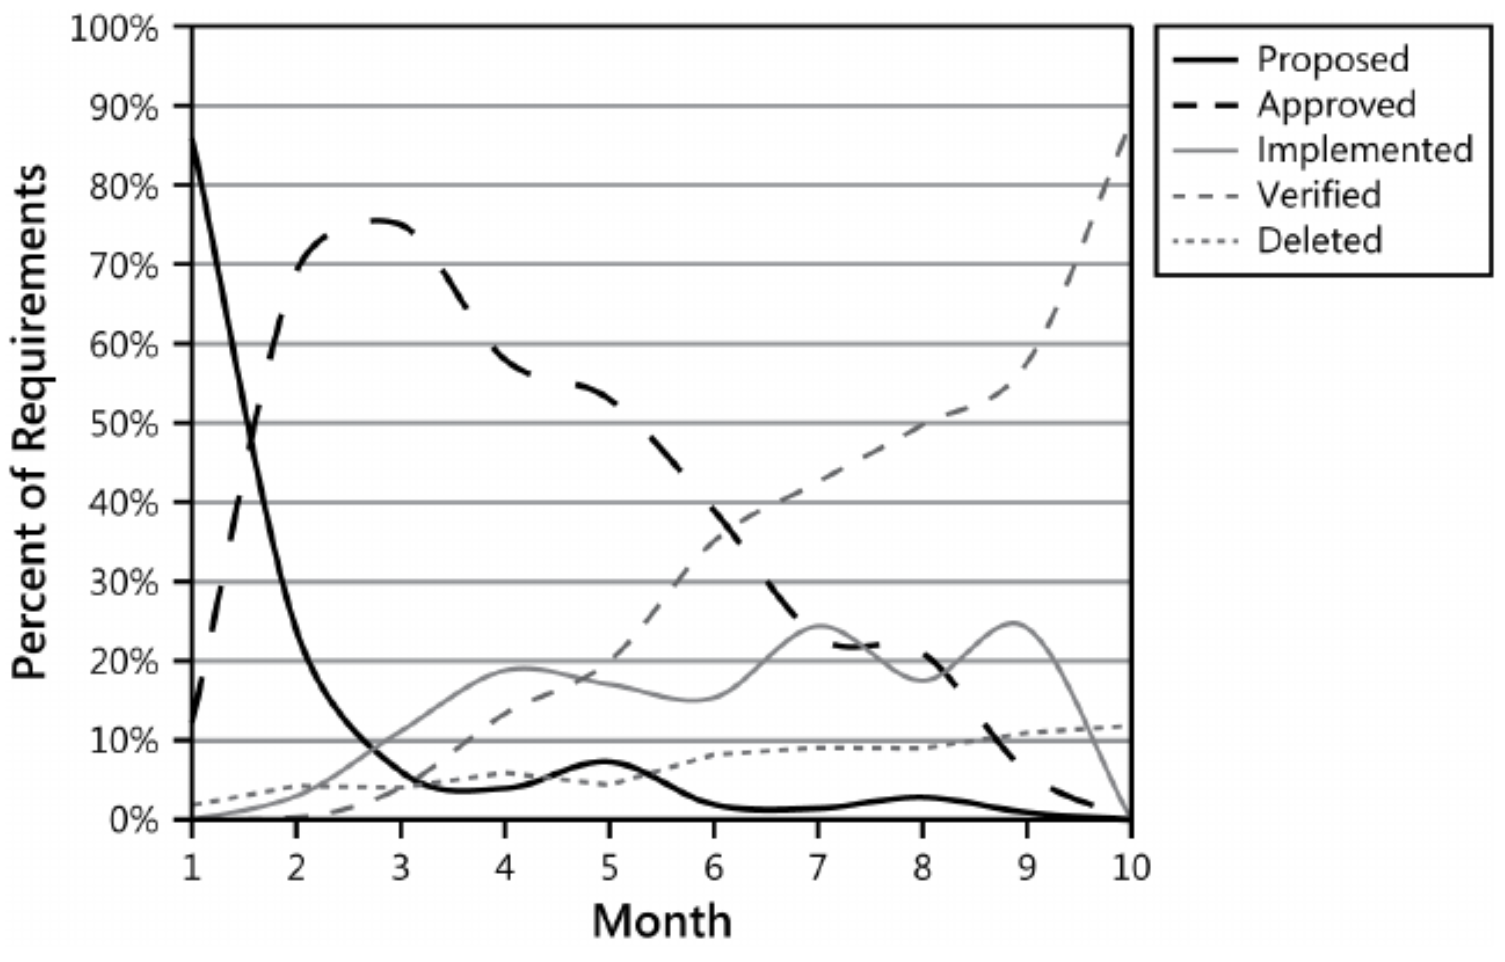
\includegraphics[width=0.8\textwidth]{burndown.png}
        \end{center}
    \end{frame}

    \begin{frame}
        \frametitle{Связь с другими видами деятельности}
        \begin{center}
            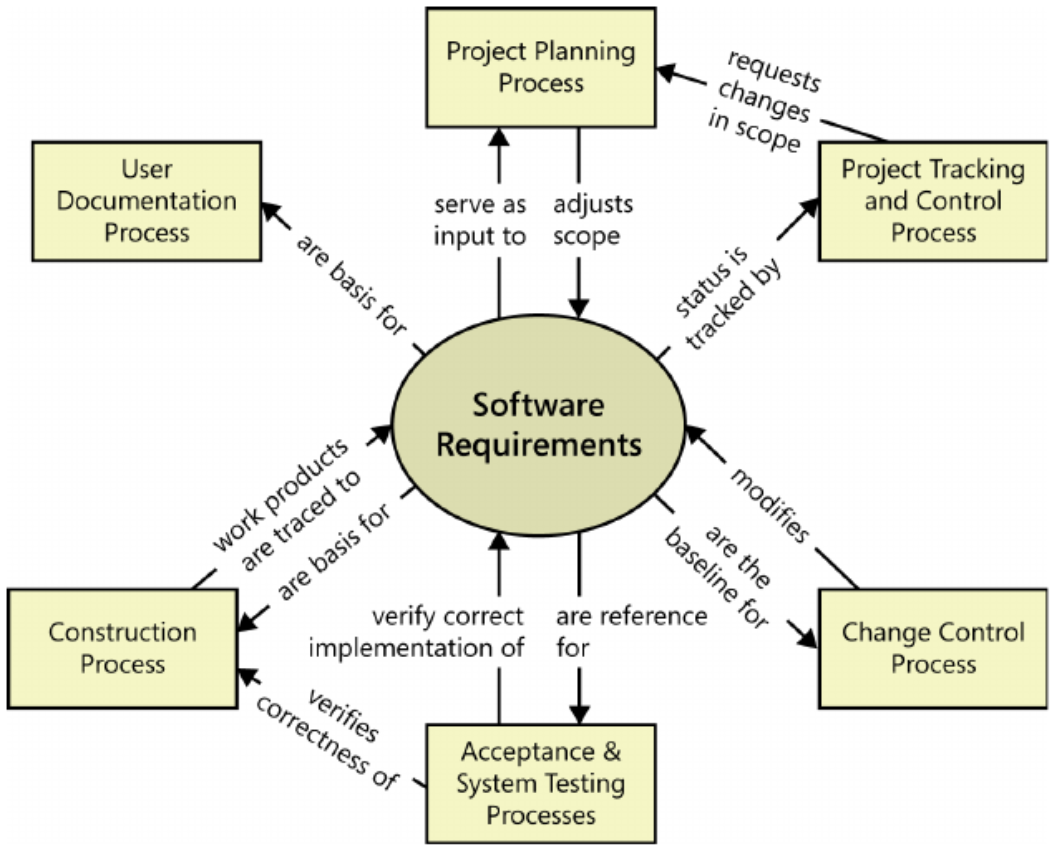
\includegraphics[width=0.7\textwidth]{requirementsAndOtherActivities.png}
        \end{center}
    \end{frame}

    \begin{frame}
        \frametitle{Доп. информация}
        \begin{columns}
            \begin{column}{0.5\textwidth}
                \url{https://stepik.org/course/1128/}
            \end{column}
            \begin{column}{0.5\textwidth}
                \strut
                
\includegraphics[width=0.8\textwidth]{bookCover.png}
            \end{column}
        \end{columns}
    \end{frame}

\end{document}
